\subsection{Переходные процессы в нелинейных цепях}



Метод переменных состояния основывается на упорядоченном составлении и решении системы дифференциальных уравнений первого порядка, которые разрешены относительно производных, т.е. записаны в виде, наиболее удобном для применения численных методов интегрирования, реализуемых средствами вычислительной техники.

Количество переменных состояния, а следовательно, число уравнений состояния равно числу независимых накопителей энергии.

К уравнениям состояния выдвигаются два основных требования:

-независимость уравнений;

-возможность восстановления на основе переменных состояния (переменных, относительно которых записаны уравнения состояния) любых других переменных.

Первое требование удовлетворяется специальной методикой составления уравнений состояния, которая будет рассмотрена далее.

Для выполнения второго требования в качестве переменных состояния следует принять потокосцепления (токи в ветвях с индуктивными элементами) и заряды (напряжения) на конденсаторах. Действительно, зная закон изменения этих переменных во времени их всегда можно заменить источниками ЭДС и тока с известными параметрами. Остальная цепь оказывается резистивной, а следовательно, всегда рассчитывается при известных параметрах источников. Кроме того, начальные значения этих переменных относятся к независимым, т.е. в общем случае рассчитываются проще других.

\begin{center}
	\begin{figure}[h!]
		\center{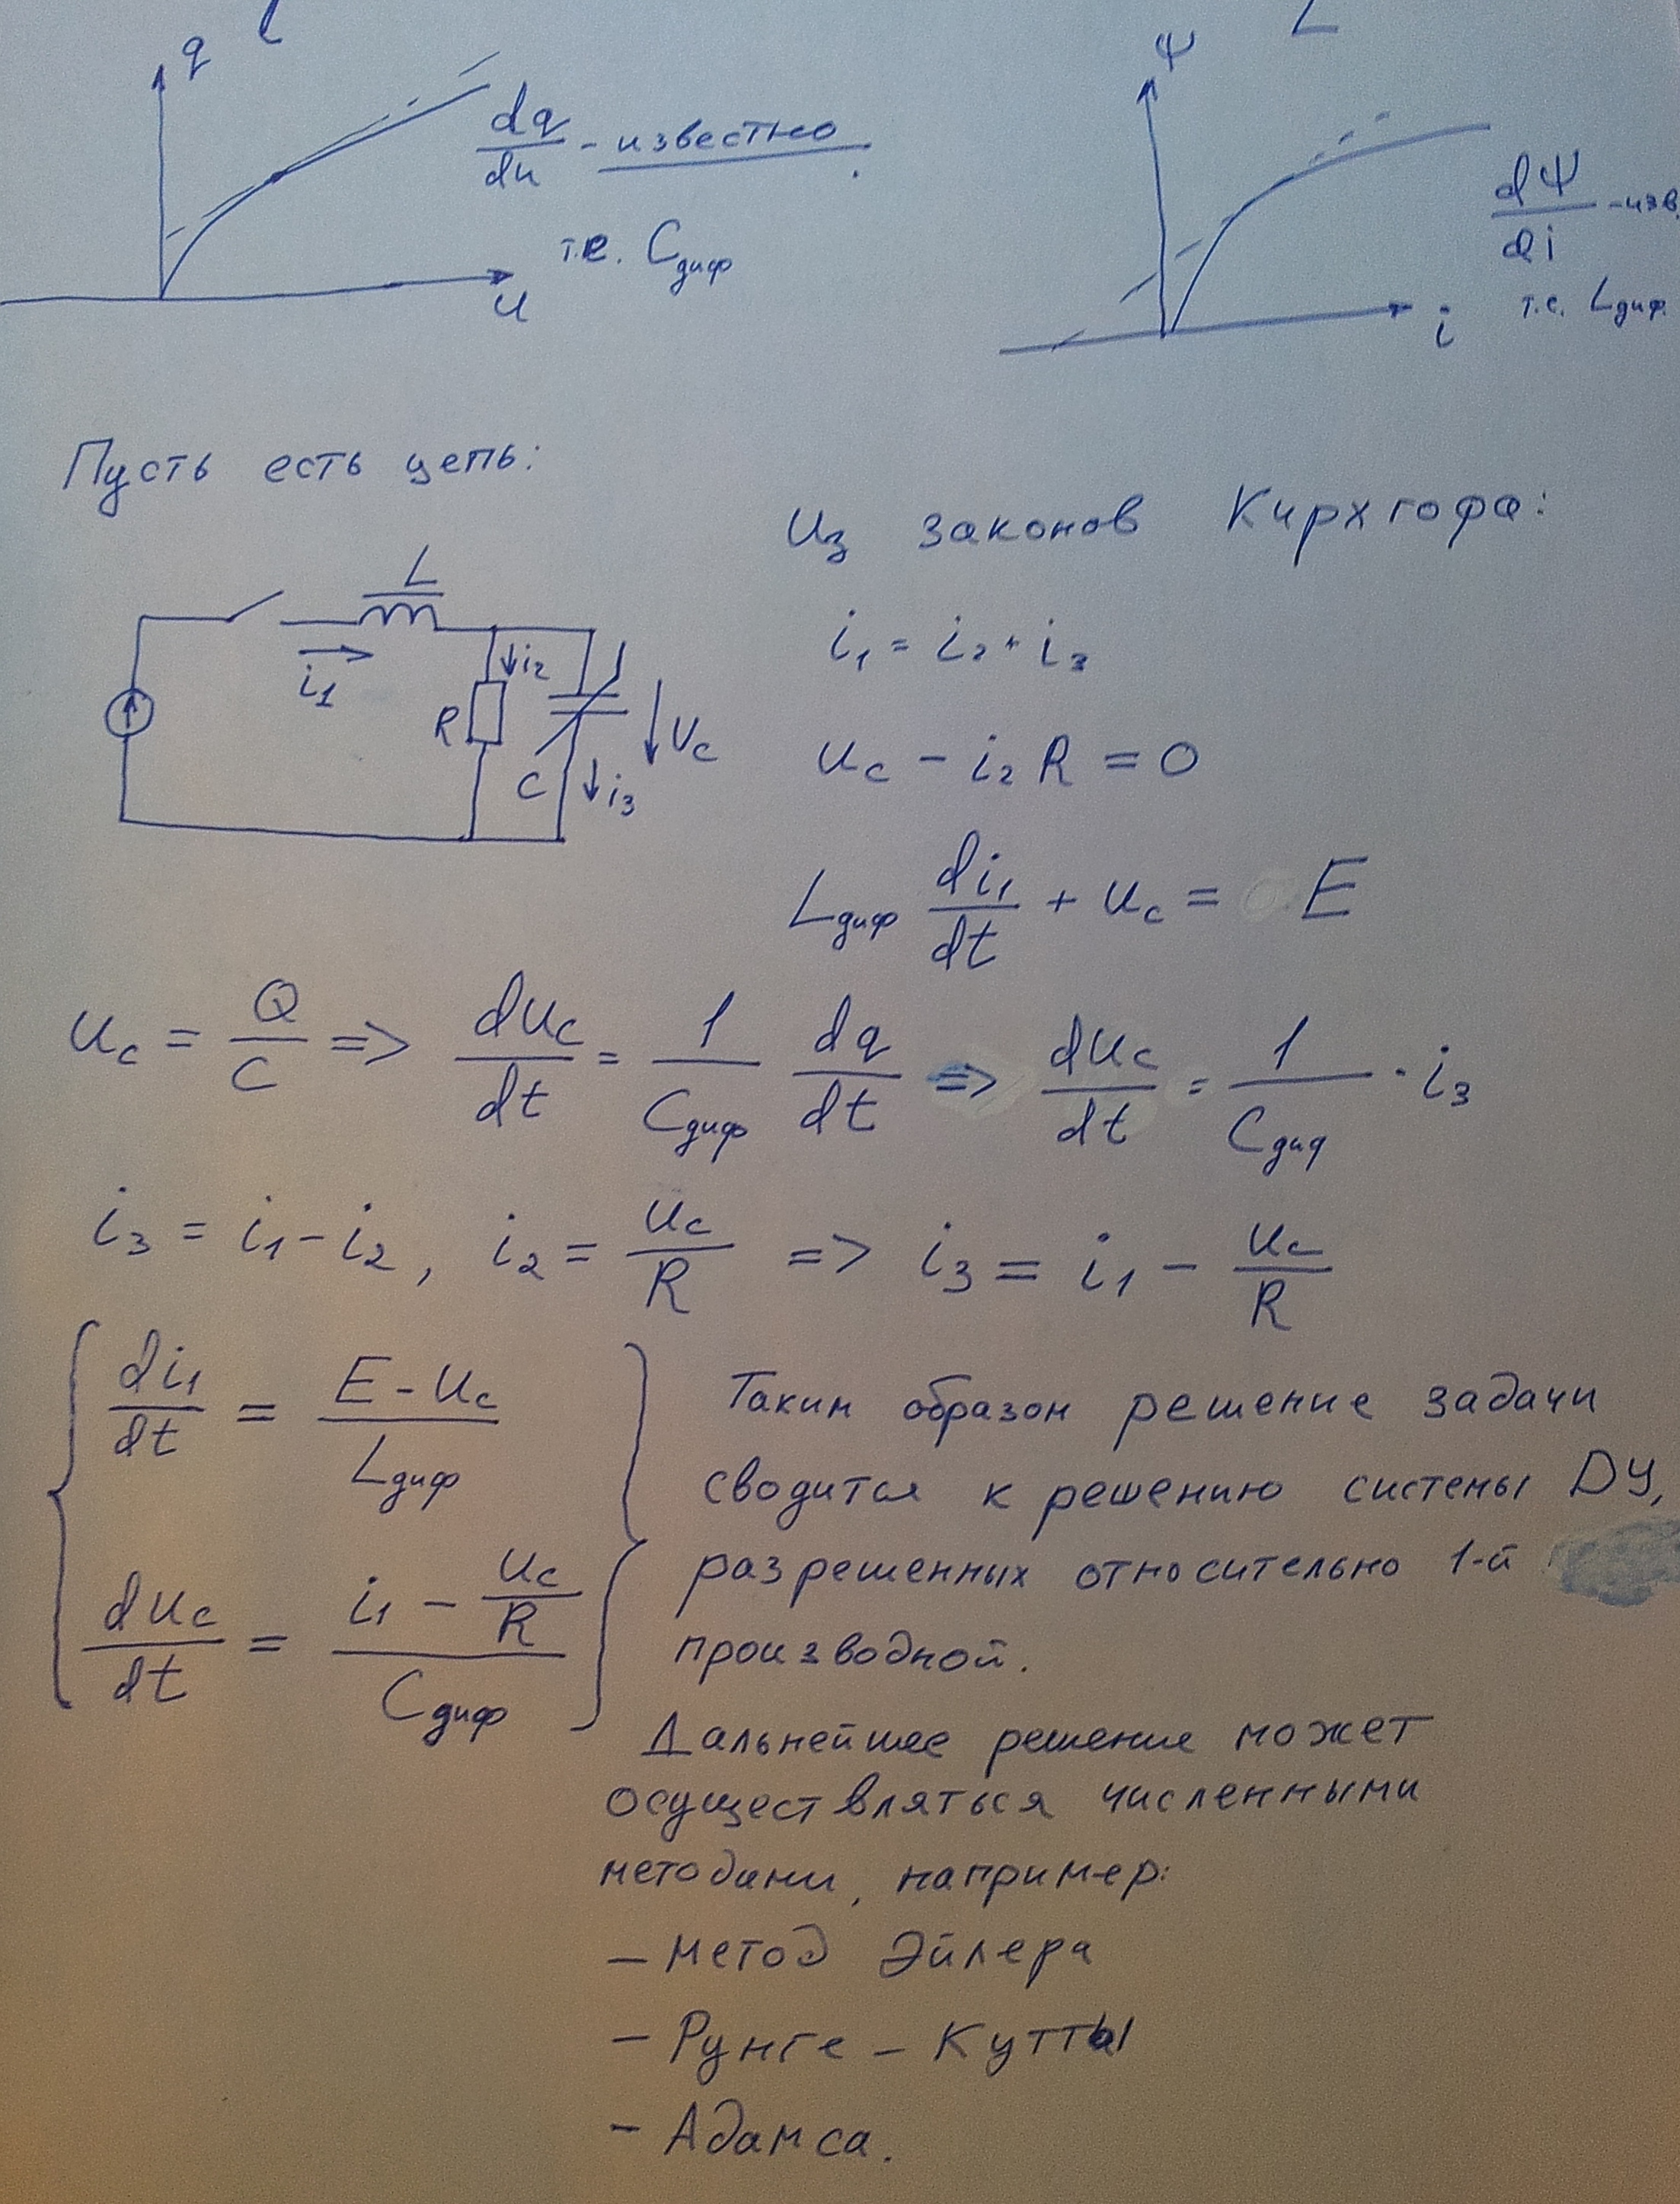
\includegraphics[scale=0.24]{state_varible.jpg}}
		\caption{Пример метода переменных состояния}	
	\end{figure}
\end{center}


\pagebreak
